% !TeX spellcheck = en_GB

\section{\protect{\emoji{thinking-face}} The problem of \textit{adversarial robustness}}{

    \begin{frame}{\protect{\emoji{thinking-face}} \textit{Adversarial inputs and attacks}}
        The last shown picture is an example of
        \hfill\break
        \begin{block}{\textit{Adversarial Input}}
            An \textit{input} is said to be \textit{adversarial} to a machine learning system if it alters its \alert{reasonably} expected behaviour\footnote{Usually from the \textit{P.o.V.} of the user(s).}. Also called \textit{adversarial attack}, stressing the intentional\footnote{Which is not a strict requirement, though!} crafting of it.
        \end{block}

    In the specific case of a classifier: produce a \textit{misclassification}.
    \end{frame}


    \begin{frame}{\protect{\emoji{thinking-face}} Why studying \textit{adversarial robustness}?}

        We live in times where a growing portion of even \textit{high-stakes} \alert{decisions} is \alert{delegated} to autonomous systems (\textit{e.g.} \textit{HR} selection, insurance, health, fraud detection, \etc\dots).\\$\rightarrow$ The example of \textit{Lemonade} \protect{\emoji{lemon}}

        \underline{Purely \textit{technical} reasons}
        \begin{itemize}
            \item Harden \textit{ML/DL} systems against \alert{misuse} and \textit{input-tampering};
            \item Assess (and \textit{\alert{patch}!}) behaviour where it the most fragile.
        \end{itemize}

        \underline{\textit{Legal / ethical / social} reasons}
        \begin{itemize}
            \item To ensure \alert{compliance} with regulatory frameworks or coordinated initiatives thereof;
            \item Increase understanding, transparency, and societal \alert{trust}.
        \end{itemize}

        \underline{Broader-reaching goals}
        \begin{itemize}
            \item Use \textit{robustness} as a lens through which to study \textit{\alert{neurocognitive} phenomena}.
        \end{itemize}
    \end{frame}

    \begin{frame}{\protect{\emoji{thinking-face}} Where things \textit{go awry}: the \textit{Manifold Hypothesis} (I)}

        An intuitive geometrical characterisation of \textit{adversarial attacks} can be done in the light of the

        \begin{block}{\textit{\alert{Manifold} Hypothesis}}
            \textit{Natural} high-dimensionally-coded data lie on (a) \alert{low-dimensional} manifold(s), immersed within the high-dimensional allowed \textit{code space}.
        \end{block}

    This partitions the \textit{code space} in \textit{four} regions:
    \begin{enumerate}
        \item Expected behaviour region (\textit{on-manifold});
        \item Cross-boundary adversarial region (\textit{\alert{on}-manifold});
        \item \textit{Natural} non-applicability region (\textit{\alert{along} manifold});
        \item "Negative space" adversarial region (\textit{\alert{off}-manifold}).
    \end{enumerate}

    \end{frame}

    \begin{frame}{\protect{\emoji{thinking-face}} Where things \textit{go awry}: the \textit{Manifold Hypothesis} (II)}
        \begin{center}
            "A picture is worth thousand words". (\textit{Here's $2\times10^3$!})
        \end{center}

        \begin{minipage}[c]{0.49\textwidth}
            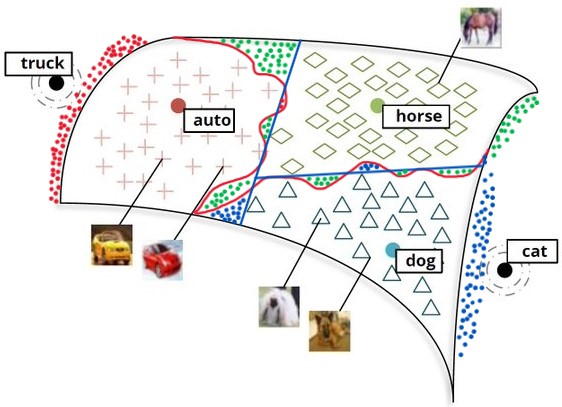
\includegraphics[width=1\textwidth, height=1\textheight, keepaspectratio]{manifold-hyp}
        \end{minipage}
        \begin{minipage}[c]{0.49\textwidth}
            \vspace{0pt}
            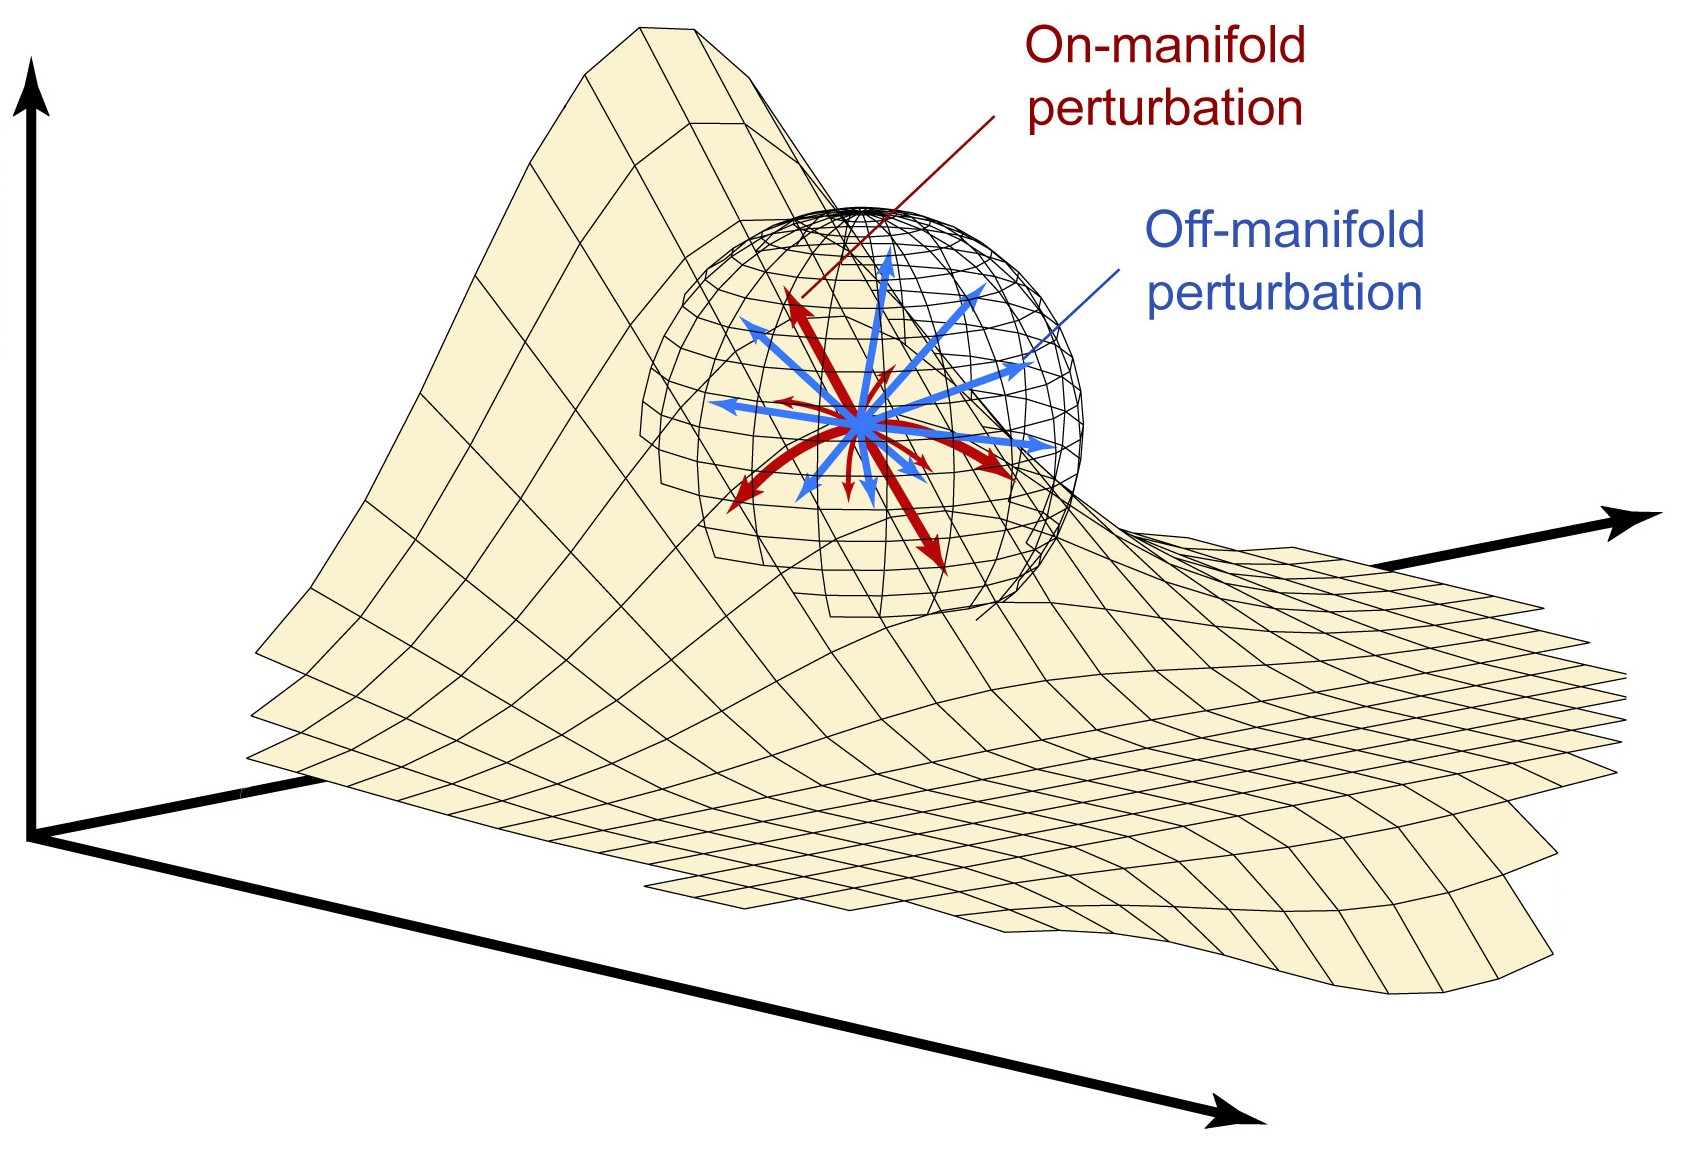
\includegraphics[width=1\textwidth, height=1\textheight, keepaspectratio]{manifold_ball_perturbations}
        \end{minipage}

    \end{frame}

    \begin{frame}{\protect{\emoji{thinking-face}} A (more) precise definition of \textit{robustness}}

        We can always reformulate the problem of \textit{adversarial inputs} as one of \textit{\alert{adversarial perturbations}}, \textit{i.e.}
        $$ \vec{x}_{\text{adversarial}} \coloneq  \vec{x}_{\text{legitimate}} + \alert{\vec{p}}$$

        leading to the following

        \begin{block}{Definition: \textit{\alert{$\epsilon$}-perturbative adversarial attack against classifier $\netw{N}$ in $x_0 \in \mathbb{I}$, \wrt $\normof{\cdot}$}}
            Any $\vec{x^{\star}} \coloneq \vec{x_0} + \vec{p} \text{ | } \netw{N}(\vec{x^{\star}}) \neq \netw{N}(\vec{x_0})$ and $\normof{\vec{p}} < \epsilon$
        \end{block}

    \underline{Minimal systematics}:
    \begin{itemize}
        \item \textit{black box} vs. \textit{\alert{white box}};
        \item \textit{targeted} vs. \textit{\alert{untargeted}}.
    \end{itemize}

    Needless to say: \textit{the world is not so simple; however...}
    \end{frame}

    \begin{frame}{\protect{\emoji{thinking-face}} \textit{How it's done}: attacks}

        \underline{\textit{White-box} scenario}
        \begin{itemize}
            \item Direct, \alert{gradient}-based (\textit{e.g.} \texttt{FGSM} \& derived);
            \item Iterative, \alert{gradient}-based (\textit{e.g.} \texttt{PGD}, \texttt{DeepFool});
            \item Specific response-elicitation methods (\textit{e.g.} \textit{k-pixel} attack, \textit{noisy \texttt{FGSM}}).
        \end{itemize}

        \underline{\textit{Black-box} scenario}
        \begin{itemize}
            \item \textit{Gradient-free} optimisation schemes;
            \item Direct-sampling \textit{generative} methods (\textit{e.g.} \texttt{AdvGAN(++)});
            \item \textit{White-box} methods towards \alert{surrogate} models (\textit{e.g.} \textit{Tramèr ensemble}).
        \end{itemize}

        \begin{block}{Definition: \textit{Universal Attack} (scheme)}
            A scheme for generating adversarial attacks able to reach \alert{any} point within the (chosen norm-induced) ball of radius $\epsilon$ ($\forall \epsilon$) centred in any \textit{legitimate} input point. Related: \textit{information \alert{optimal} attack}.
        \end{block}
    \end{frame}

    \begin{frame}{\protect{\emoji{thinking-face}} \textit{How it's done}: defences}

        That of \textit{adversarial robustness} research is a typical open, \textit{ladder-and-fence} scenario...\\
        With an even greater variability in defences:
        \begin{itemize}
            \item \textit{Adversarial training}: \alert{augment} $\mathbb{T}$ with correctly-labelled adversarial inputs (\textit{e.g.} \texttt{IAT});
            \item Adversarial detection: \alert{identify and handle} anomalous inputs (\textit{e.g.} \textit{\texttt{GAN}-discriminator anomaly detection});
            \item Adversarial purification: \alert{recover} \textit{clean} inputs from perturbed ones (\textit{e.g.} \texttt{PuVAE}, \texttt{DefenseGAN}, \textit{diffusion-based purification});
            \item \alert{Inference}-time defences: \textit{e.g.} \textit{filter} based, \textit{test-time augmentation} based, \etc;
            \item Robustly-\alert{structured} learning (\textit{e.g.} \textit{Parseval Networks});
            \item Paradigmatic shifts (\textit{e.g.} \textit{Bayesian} NNs).
        \end{itemize}
    \end{frame}

    \begin{frame}{\protect{\emoji{brain}} But, \textit{at the end of the day}...}

        No optimal, universal defence! Many \textit{case-by-case} results, many \textit{trade-offs}, practically no \textit{robust-by-design} applicable solution.
        \hfill\break

        \begin{block}{A remark}
            But... have \textit{\alert{you}} ever experienced an \textit{adversarial(-like) phenomenon?}
        \end{block}

    \end{frame}


}